\chapter{Estado de la cuestión}
\noindent
En este capítulo se describen las características más importantes acerca de otros proyectos que se utilizan actualmente para la gestión de dietas.

\subsubsection{Indya}
Es una aplicación \cite{app_indya} (ver figura \ref{fig:indya_app}) para iOS y Android que genera un menú semanal completo para seguir durante un mes. A su vez ayuda a realizar la lista de la compra, indicando los ingredientes y calorías que se necesitan cada semana para rendir al máximo. La aplicación cuenta a su vez con un nutricionista, que recibe los datos de un usuario y reajusta su planificación para conseguir los objetivos.
\begin{figure}[H]
    \centering
    \subfigure{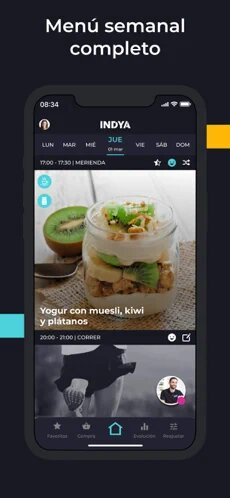
\includegraphics[width=0.3\textwidth]{Images/Capitulo2/indya.jpg}}
    \subfigure{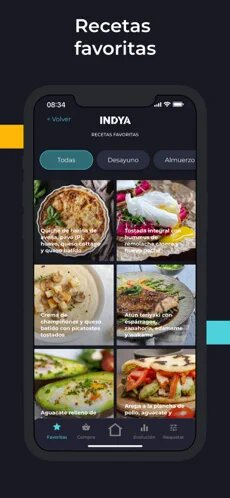
\includegraphics[width=0.3\textwidth]{Images/Capitulo2/indya2.jpg}}
    \caption{Menú principal de la aplicación \textbf{Indya}}
    \label{fig:indya_app}
\end{figure}

\subsubsection{Oorenji}
Es una aplicación \cite{app_orenji}(ver figura \ref{fig:orenji_app}) donde a partir de los gustos, alergias, del perfil físico y psicológico del usuario, genera una dieta totalmente adaptada para poder conseguir todos los objetivos. Además se puede contactar con un nutricionista de forma \textit{online} para obtener asistencia. La aplicación propone además una serie de retos para ayudar a cumplir los objetivos.
\begin{figure}[H]
    \centering
    \subfigure[Vista de dietas]{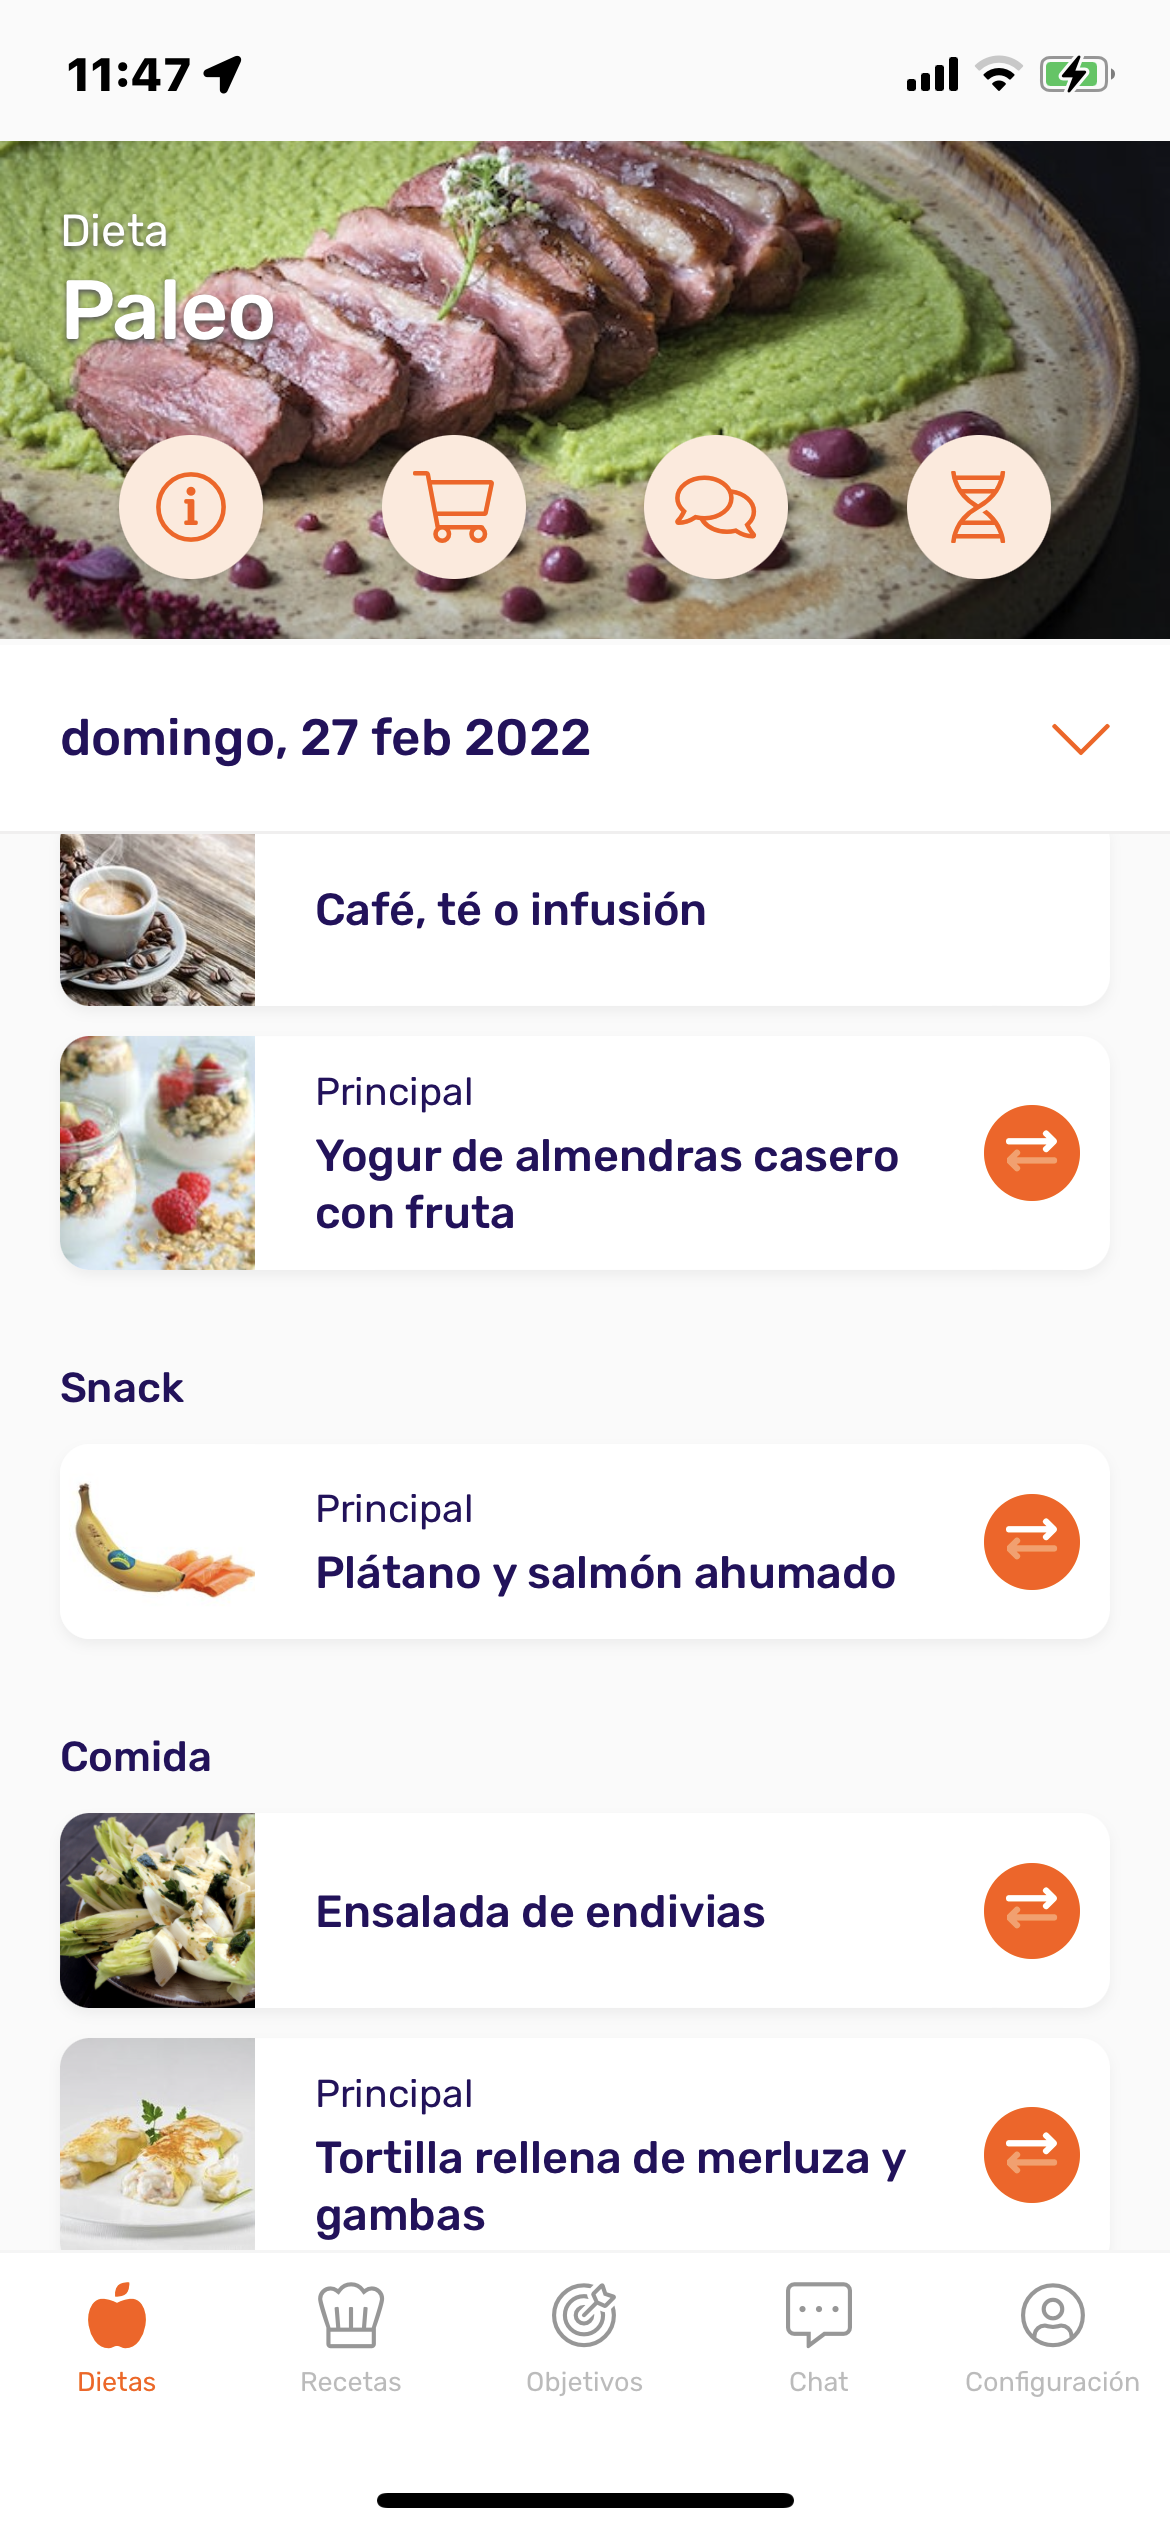
\includegraphics[width=0.4\textwidth]{Images/Capitulo2/orenji.png}}
    \subfigure[Vista detallada de una dieta]{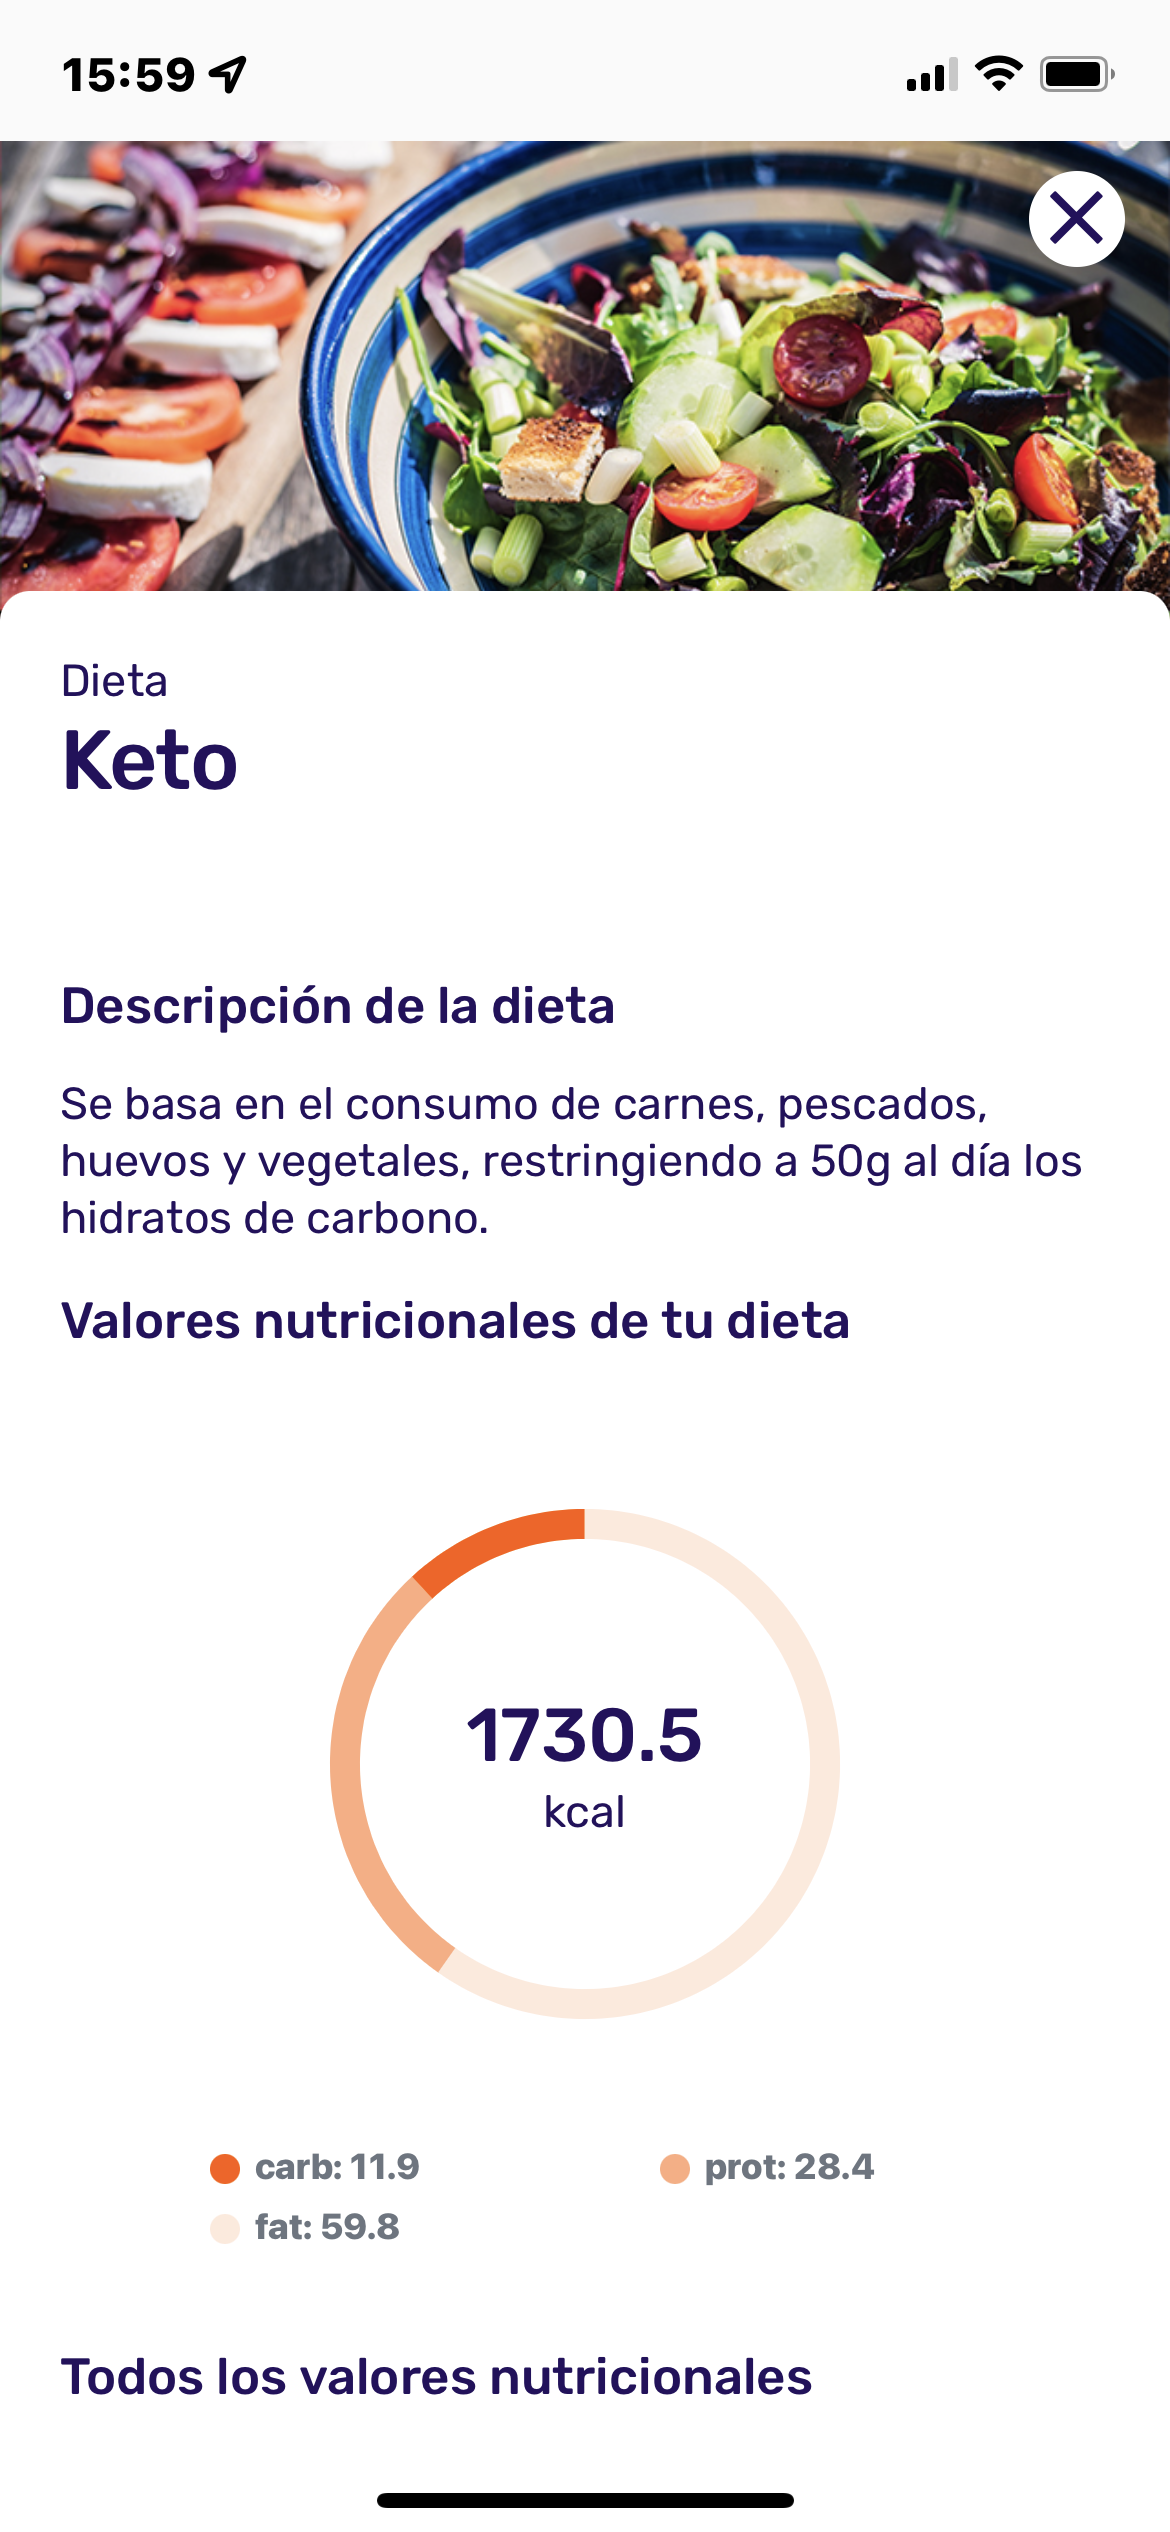
\includegraphics[width=0.4\textwidth]{Images/Capitulo2/orenji2.png}}
    \caption{Diferentes vistas de la aplicación \textbf{Oorenji}}
    \label{fig:orenji_app}
\end{figure}

\subsubsection{FatSecret}
Es una aplicación \cite{app_fat_secret} (ver figura \ref{fig:fatsecret_app}) para Android que además de contabilizar las calorías ingeridas y quemadas, puede analizar el código de barras de los alimentos. Además, ayuda a controlar la cantidad de los tres macronutrientes (proteínas, carbohidratos y grasas) que se ingieren diariamente.
\begin{figure}[H]
    \centering
    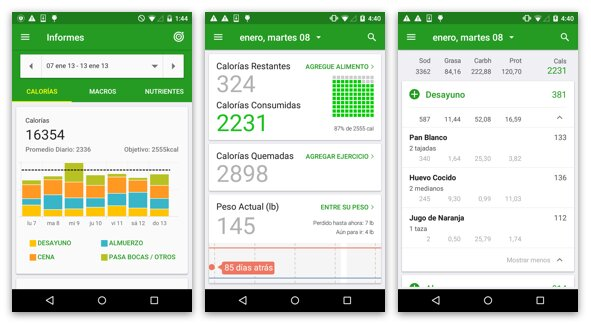
\includegraphics[width=\textwidth]{Images/Capitulo2/fatsecret.jpg}
    \caption{Distintas pantallas de la aplicación \textbf{FatSecret}}
    \label{fig:fatsecret_app}
\end{figure}


\subsubsection{Nootric}
Es una aplicación \cite{nootric} (ver figura \ref{fig:nootric_app}) en la que se pueden realizar diferentes planes nutricionales con recetas. Incluye recetas de cocina, guías y consejos para adelgazar y una lista de la compra por cada semana del mes. También dispone de una versión de pago, la cual cuenta con un mayor número de planes nutricionales así como un seguimiento a medida por parte de un nutricionista.
\begin{figure}[H]
    \centering
    \subfigure[Vista del menú]{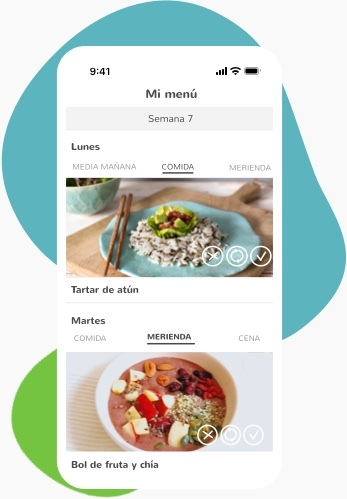
\includegraphics[width=0.3\textwidth]{Images/Capitulo2/nootric_1.jpg}}
    \subfigure[Vista de entrenamientos]{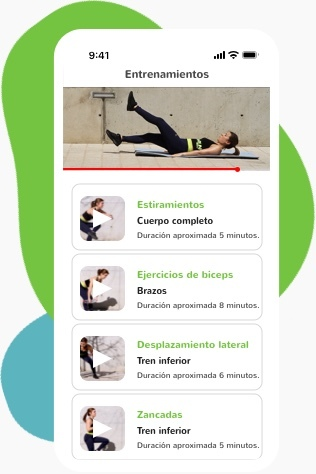
\includegraphics[width=0.3\textwidth]{Images/Capitulo2/nootric_2.jpg}}
    \caption{Distintas pantallas de la aplicación \textbf{Nootric}}
    \label{fig:nootric_app}
\end{figure}


\subsubsection{Fitia}
Es una aplicación \cite{fitia} (ver figura \ref{fig:fitia_app}) en la que se puede visualizar cada una de las comidas del día además de contar las calorías y calcular los nutrientes presentes en las recetas que ofrece. Dispone de varias opciones para alcanzar el objetivo deseado, desde aumentar masa muscular, reducir grasa corporal o simplemente mantener una dieta sana y saludable.

\begin{figure}[H]
    \centering
    \subfigure[Plan nutricional]{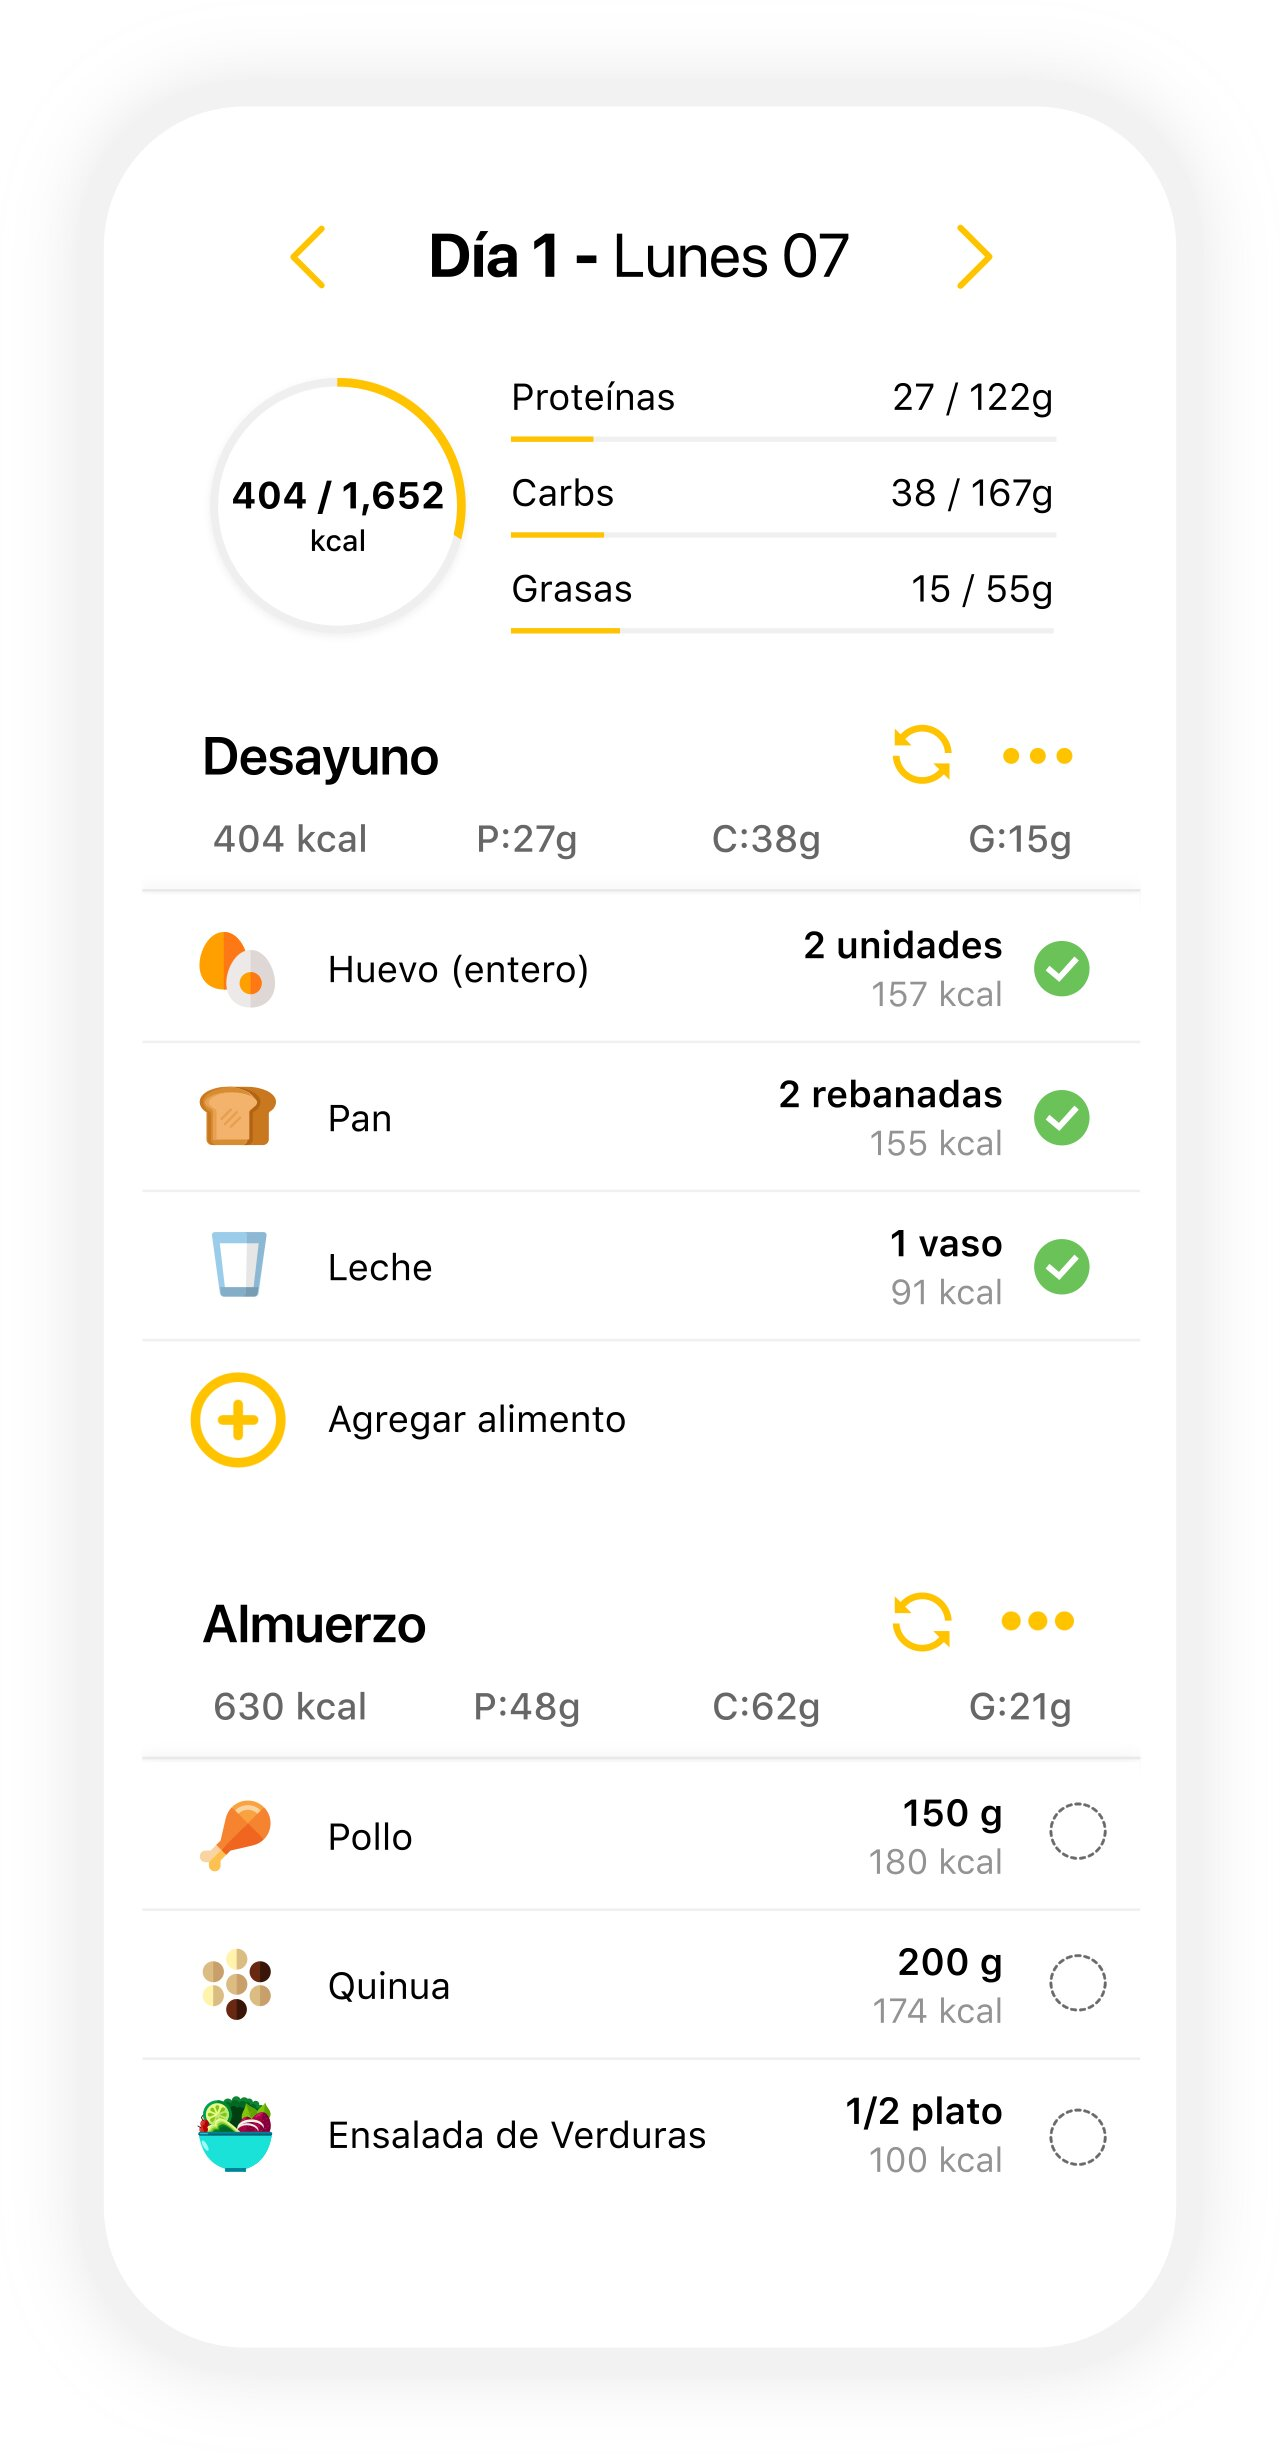
\includegraphics[width=0.4\textwidth]{Images/Capitulo2/plan-nutricional.jpg}}
    \subfigure[Información alimentaria]{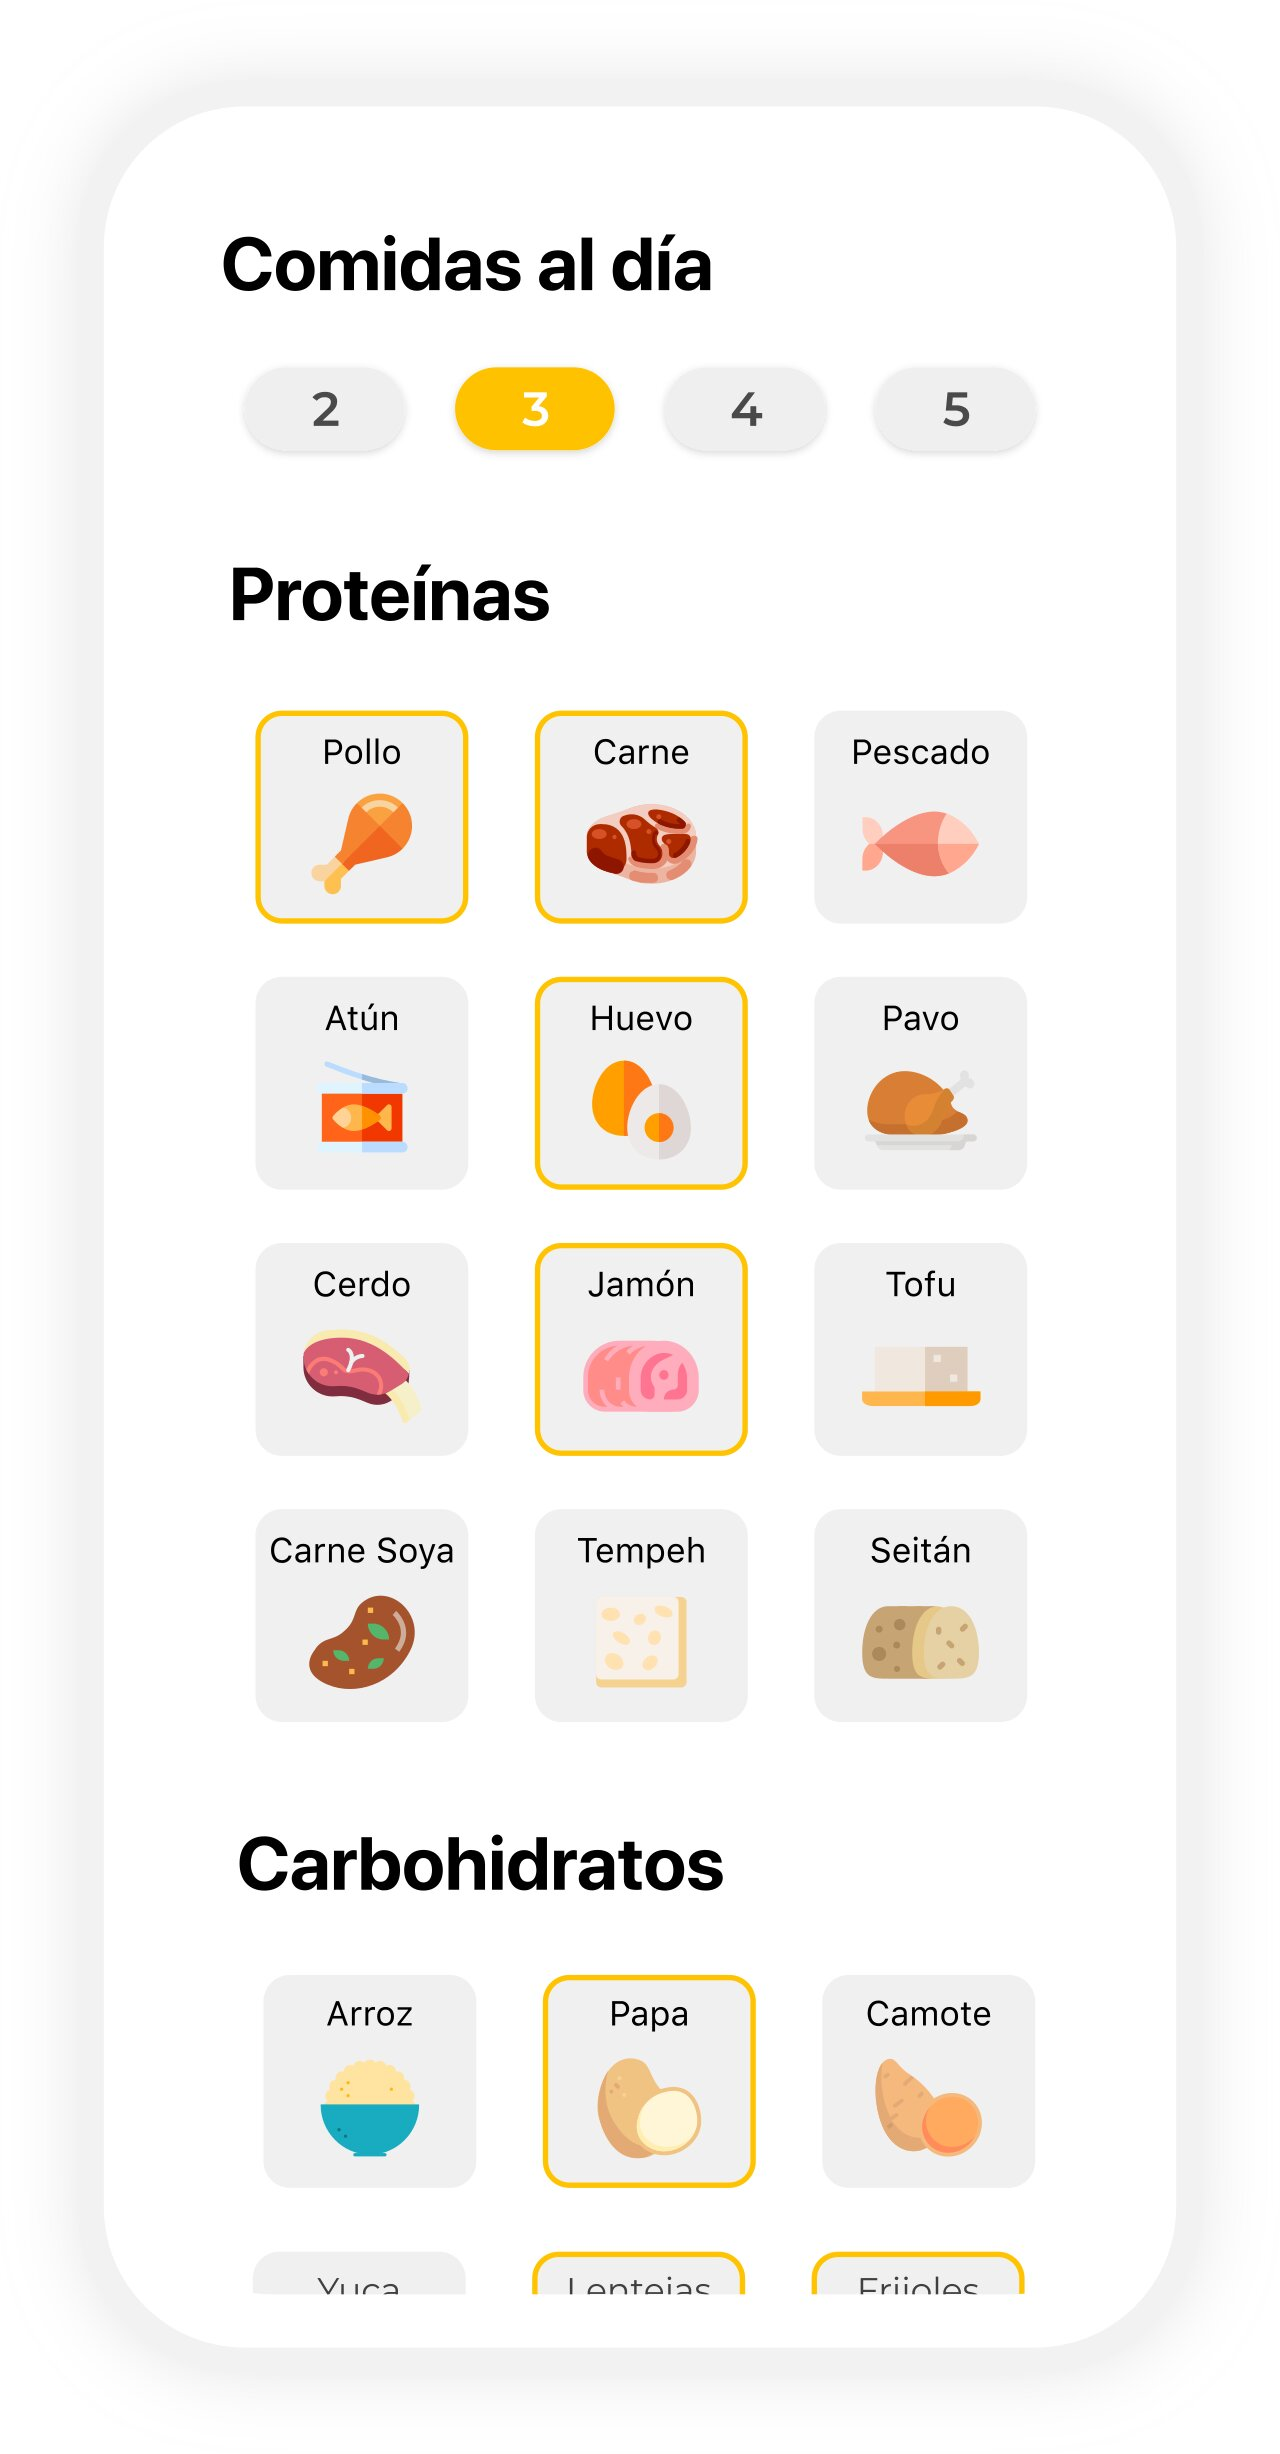
\includegraphics[width=0.4\textwidth]{Images/Capitulo2/alimentos-proteinas-carbohidratos-grasas.jpg}}
    \caption{Distintas pantallas de la aplicación \textbf{Fitia}}
    \label{fig:fitia_app}
\end{figure}